% This is the chapter 'Electricity-Foundations' to the "Hodgkin-Huxley neuron model V2.0 book"
% Last edited 2026.06.23

\ifx\magyar\undefined

\section[Why different]{Why ions' electricity is different\label{sec:PHYSICS_ElectricWhyDifferent}}

\else

\section[Miért más]{Miért más az ionok elektromosságtana\label{sec:PHYSICS_ElectricWhyDifferent}}

\fi

This section recalls dichotomies discussed in section~\ref{sec:Physics-Dichotomies} from the viewpoint of electricity.
Electricity is one of the fundamental disciplines of classical physics. It operates with concepts such as charge, current, voltage; furthermore, their
spatial or temporal change described by their gradients (spatial or temporal derivatives).
Physical and biological electricity are similar, but not identical.
The former was already an established discipline when the latter
started to discover that biological objects also show signs of electric processes occurring inside them.
Of course, the already available concepts, laws, measurement devices and procedures were taken over, and based on the resemblance between those two kinds of electricities, their identity was and is assumed.
The laws of physical electricity, in most cases, describe also biological electricity to some measure. 
However, in some cases, there are drastic differences between them.
Not considering those differences leads to misunderstandings and wrong conclusions.

Physical electricity operates with concepts of ideal (voltage or current) generators, ideal (that is single-substance) charge carriers, and discrete components, connected by ideal conducting wires.
The wires are passive components, just connect
the discrete components and the electric phenomena happen in the 
discrete elements, with one idealized feature.
Physical electricity inherited the Newtonian picture that everything happens simultaneously and it applies a hybrid picture.
It considers that no delay exists on the connecting wires, although charge passes in the current.  
The current is defined as temporal change of charge,
but it is explicitly considered only in the slighty non-ordinary 
phenomena capacitance, inductance and impedance; it is considered
as instant in the phenomenon called resistance.
\index{ordinary laws}
In biological electricity, neither of the above  disciplinary concepts
can be interpreted in unchanged form, they must be reinterpreted. The charges are moved not necessarily by an electric field,
but their movement is interpreted as current (and, simultanously, as mass transport) furthermore,
that movement creates change in the potential (as well as in the concentration), due to the limited resources.
\index{limited resource}
Since the charge carriers are slow,
local, instead of global, potentials must be used. 
The integral forms of laws of electricity are not valid in the form
we used to in physical electricity. The charge (and mass) conservation
are valid only in the global sense; while in classical physics, with its concept 'instant interaction', local and global coincide.
%
Fortunately, physiology inherited the ambititon from physics to measure its subject, together with the measurement methodologies and devices. Unfortunately,
as we detail in section~\ref{sec:PHYSICS_MEASURING}, measuring living matter (because of its "special construction") requires at least considerable care,
sometimes different methodologies and appropriate interpretation; including the understanding of the special kind of electricity it applies.

The different charge transmission mechanism introduces another important difference, the relation to thermodynamics.
In physical electricity, the medium is a solid, where the electrons heavily interact with the nodes in the solid (forming a kind of 'electron cloud'). In a good approximation, they are not comprising free and independent particles, so their phenomena are not related to thermodynamics. The ions, in contrast,
are nearly independent, so they would be described by thermodynamics.
However, they are simultanously also charged particles, so they are governed also by the laws of electricity. These two circumstances together represent a case which is not belonging to either dicipline.
More precisely, neither of the two disciplines can describe the
phenomena without the other.
The case is somewhat similar to the case when an ion moves in simultanously applied electric and magnetic fields,
and it is considerably different in that the thermodynamic interaction also represents a mass transport,
inseparably, so the driving force is the sum of the thermal and electric gradients.
\textit{The real complication and difference is, however, that the interactions have different speeds.}
However, it is not a different physics ("or whatnot").
It is only using different laws for the different environment
from the same first principles.


 
\section[Concepts]{Fundamental concepts\label{sec:PHYSICS_ELECTRICFundamental}}  

The disciplinarily separated sience defines \href{http://hyperphysics.phy-astr.gsu.edu/hbase/electric/elefie.html#c1}{electricity's concepts}
through forces and infinitely small test charge. In living matter,
neither is valid in an unchanged form: constraints and physical/chemical additional forces are present, furthermore, the charges of the carriers are not
negligible compared to the charges that generate the field acting on the charges. Furthermore, \textit{since the carriers have mass, 
one cannot apply laws of disciplinary electricity since they are valid for "slow" currents in a different form}. One may have fundamental problems with the mathematical descriptions: 
the discrete nature of charge carriers question marks the differentiability of the corresponding functions,  
the charge-mass dichotomy of ions the interpretation of 
\hyperlink{PartialDerivative}{partial derivatives}, furthermore, the simultaneity of different phenomena.
\index{dichotomies in science}
\index{differentiability}
\index{partial derivative}
\index{simultaneity}


\ifx\magyar\undefined
\subsection[Charge]{Charge\label{sec:Electricity-Charge}}

\else

\subsection[Töltés]{Töltés\label{sec:Electricity-Charge}}

Az ion tovább már nem egyszerűsíthető tulajdonsága, hogy
töltést hordoz
\fi


\ifx\magyar\undefined
\subsection[Field]{Electric field\label{sec:Electricity-Field}}

\else

\subsection[Erőtér]{Elektromos erőtér\label{sec:Electricity-Field}}

\fi

%It is a common fallacy in physiology that the applied potential $U$ generates
%a current. Instead, its gradient ($E=U/d$) has the effect, where $d$ is the distance, for example, between the clamping point and the membrane or the \gls{AIS}.

\ifx\magyar\undefined
\subsection[Voltage]{Voltage\label{sec:Electricity-Voltage}}

\else

\subsection[Feszültség]{Feszültség\label{sec:Electricity-Voltage}}

Az ion tovább már nem egyszerűsíthető tulajdonsága, hogy
töltést hordoz
\fi

\ifx\magyar\undefined
\subsection[Current]{Current\label{sec:Electricity-Current}}

\else

\subsection[Áram]{Feszültség\label{sec:Electricity-Current}}

Az ion tovább már nem egyszerűsíthető tulajdonsága, hogy
töltést hordoz
\fi

\subsubsection{Ionic currents in a cell\label{sec:Electricity-IonicCurrent}}


On a microscopic scale, a charge generates a potential field that acts on other charges. It is a common fallacy in physiology that a "potential field travels": neither potential nor current changes without a physical movement of charges. In a conducting wire filled with ions (the solids have a different current transfer mechanism), there are free charges; their
number per unit volume is given by $n$, and $q$ is the amount of
charge on each carrier. If the conductor has a cross-section of $A$,
in the length $dx$ of the wire, we have charge $dQ=q*n*A*dz$. If the charges move with a macroscopic speed $v=\frac{dz}{dt}$, 
at the macroscopic level, we define the current $I$ as the charge moved per unit of time as
\begin{equation}
	I=\frac{dQ}{dt}=q*n*A*v\label{eq:DriftCurrent}
\end{equation}
The effect was hypothesized at the very beginning: "it seems difficult to escape the conclusion that the changes
in ionic permeability depend on the movement of some component of the
membrane which behaves as though it had a large charge or dipole moment."
"it is necessary to suppose
that there are more carriers and that they react or move more slowly"~\cite{HodgkinHuxley:1952}. The charged ions, attracted by the opposite charges on the other plate and repelled toward the single exit point \gls{AIS}, really move slowly and behave as if they were a component of the membrane.

Notice that if any of the factors is zero, the macroscopic current
$I$ is zero. \textit{Microscopic carriers must be present in the volume},
and have charge, the cross section must not be zero, and the charge
carriers must move with a potential-assisted speed, which needs an
electrical field generated by the system, see Eq.(\ref{eq:IonicForces}).
When there is no constraint force, the thermodynamic and electrical forces will produce an effective force that moves the ions.
That is, the ions can move without an external electrical field, as experienced
in biological systems. 
One of the fundamental mistakes by \gls{HH} was neglecting the Coulomb force in ion-electrical interactions and assuming that diffusion processes or ideal electrical batteries create the electrical potential.

In biological systems, where ions represent the "current", it is either a native current (without an external potential) or an artificially injected current or potential generating a current.
This way, the current is consistently accompanied by a change in concentration gradient, as the moving ions represent both mass and charge transfer simultaneously (also, the repulsion leads to a "skin effect": in electrical wires and axons, the charge travels near
the outer surface).
The potential and current are
connected through the features of the medium (material) that hosts
our measurement. 
%One must not forget that "Unfortunately, most measuring devices in neurophysiology are precise without being accurate"~\cite{JohnstonWuNeurophysiology:1995}. So are some definitions, too.
%Definitions and measurements that are not accurate lead to incorrect results.
%They may be precise, but they are not accurate.

\subsubsection[Speed]{Current's speed\label{sec:Electricity-ion's-speed}}
According to Stokes' Law, to move a spherical object
with radius $a$ in a fluid having dynamic viscosity $\eta$, we need
a force
%
\begin{equation}
	F_{d}=6*\pi*\eta*a*v\label{eq:StokesForceOnIon}
\end{equation}

\noindent (drag force) acting on it. A (microscopical) electrical force
field $\frac{dV}{dz}$ inside the wire would accelerate the charge
carriers continuously
%
\begin{equation}
	F_{electric}=k* E(z) * q
\end{equation}
\noindent with a constant speed $v$. It is not the \emph{drift} speed because of the
electrical repulsion, it is a \emph{potential-assisted} or \emph{potential-accelerated} speed that can
be by orders of magnitude higher.  
The medium in which the charge moves shows a (macroscopic,
speed-dependent) counterforce $F_{d}$, which in steady state equals
$F_{electric}$, that is :
%
\begin{equation}
	I=\frac{k*q^{2}*A}{6*\pi*\eta*a}*n*E(z)
	\label{eq:StokesCurrent}
\end{equation}

We extend the original idea by using
\[
E(z)  = E_{electric} + E_{thermal} + E_{external}\quad in\ electrolytes
\]
that is, for living matter
\begin{align}
	E(z) & = \frac{\Delta V}{\Delta z} & in\ linear\ potential\\
	& = \frac{dV}{dz} & in\ graded\ potential\\
	& = E_{electric} + E_{(thermal)}  (+ E_{(external)}) & in\ electrolytes
\end{align}

\textit{The amount of current in a wire is not only influenced by the electric
	force field (specific resistance) but also by the number of charge
	carriers $n$.} While the latter is commonly considered constant and
part of the former, this is not necessarily the case for biological
systems with electrically active structures inside. The medium's internal
structure ("the construction) introduces significant modifications. \textit{Applying an electric
	field to a biological wire can generate varying amounts of current as the number
	of charge carriers changes due to biological effects.} For axons, we use a single-degree-of-freedom
system, a viscous damping model, so the \textit{ions will move with
	a field-dependent constant velocity in the electrical field}; so it takes time while they appear on the membrane.
The activity of potential-controlled ion channels in its wall may
change $n$ in various ways; furthermore, that change can result in
'delayed' currents during measurement, for example, in clamping, as physiological measurements witness.

If we have a concentration
$C(z)$, in the volume $A*dz$, we have $dQ=C(z)*A*dx*q$
charge, resulting in another expression for the current

\begin{equation}
	I=\frac{C_k(z)*A*dz*q}{dt}=C_k(z)*A*q*v\label{eq:ConcentrationCurrent}
\end{equation}
By combining equations (\ref{eq:StokesCurrent}) and (\ref{eq:ConcentrationCurrent}): 
\hypertarget{eq:StokesLawSpeed}{ }
\begin{equation}
	v(z)=\frac{k*q}{C_k(z)*\eta*6*\pi*a}*E(z)\label{eq:StokesSpeed}
\end{equation}

The higher the resulting space derivative (gradient) and the fewer ions that
can share the task of providing a current, the higher the speed. We hypothesized (it needs
a detailed simulation) that in the case of this charged fluid, the
electrical repulsion plays the role of 'viscosity'~\cite{VeghNonOrdinaryLawsForLife:2025}. The higher the charge
density, the stronger the force equalizing the potential; so $\eta$
is the lower, the higher the charge density (proportional to $C_{k}$).
For the sake of simplicity, we assume that the speed is proportional
to the space gradient of the local concentration and potential. Recall that \emph{our equations
	refer to local gradients only. The electrical gradient can propagate
	only with the speed of the concentration gradient}, given that only
the chemically moved ions can mediate the electrical field~\cite{VeghNonOrdinaryLawsForLife:2025}. \emph{The
	lower interaction speed limits the other interaction speed if the
	interactions generate each other.}

The dependence of the diffusion coefficient on the viscosity can be modeled by the Stokes-Einstein relation:
\index{Stokes-Einstein relation}
\begin{equation}
	\label{eq:StokesEinstein}
	D = \frac{k*T}{6*\pi*\eta*a}
\end{equation}
so we can express the speed with the diffusion coefficient $D$ and temperature $T$
\begin{equation}
	v(z) = \frac{D}{T}*\frac{q}{C_k(z)}*E(z)\label{eq:StokesEinsteinSpeeddV}
\end{equation}
We introduce \textit{a time-dependent speed gradient
	$v(z,t)$
	which plays a vital role in the processes that occur in living matter}.


It is important to remember for alternating current experiments: 
the different ions will move at different speeds
under the effect of the same $E(z,t)$, which is the function of
the local concentrations and the frequency of the alternating current.
The conduction speed sensitively depends 
on the temperature, and through it, the shape parameters~\cite{APTemperatureDependence:2012} of the \gls{AP} and especially the length of the "relative refractory" period~\cite{APTemperatureDependenceRefractory:2001}.

\subsubsection{Imitating slow currents\label{sec:SlowCurrent}}
At the dawn of finding methods for describing neuronal operation,
\gls{HH}
published high-precision measurements~\cite{HodgkinHuxley:1952}
enabling detailed testing of theories explaining the observed physiological
behavior. \emph{Their good physical model that }``movement
of any charged particle in the membrane should contribute to the total
current'' \emph{lacked considering the mutual repulsion and finite speed} of those particles (they are about 50,000 times heavier and a million times slower than the electrons, and they move in a closed space segment). Furthermore, 
they have started from the commonly used wrong assumption that conductance
is a primary electrical entity.
They could "find equations which describe the conductances with
reasonable accuracy and are sufficiently simple for theoretical calculation of the \gls{AP} and refractory period".
The "reasonable accuracy" and the need for a simple calculation method (performed on a mechanical calculator) obscured
the fact that the laws for electrons are not the same as the laws derived for ions.

As discussed in connection with Eq.~(\ref{eq:DriftCurrent}),
the current depends linearly on the number of charge carriers $n$.
The physical processes changing the number of charge carriers
also define the intensity of the currents, providing a way to imitate
slow currents by fast currents (by using current generators using special function shapes), where the spatiotemporal time course of the physical process of producing ions in the system modulates the number of charge carriers.


As an example, we discuss the case of slow current
traveling in an axon.
The ions travel a finite distance with
a finite speed, so there must be a delay between their entry and exit times. The case of switching a clamping voltage
on, to some measure, is analogous to the arrival of a spike. Initially, the axon contains
no ions. 
%The front evoked by a step function is linear because of
%the slow current. 
In the classical picture, the axonal current flows into the membrane with
capacity $C_{m}$ and increases the membrane's voltage $V_{m}$
with a time constant 
\begin{equation}
	\frac{dV_{m}}{dt}=-\frac{1}{C_{m}}I_{axon};\ V_{m}(t)=\frac{I_{wall}*(1-e^{-\alpha*t})}{C_{m}}\label{eq:MembraneCurrent}
\end{equation}
%
\noindent that generates a change in the membrane current
\begin{equation}
	\frac{dI_{m}}{dt}=\frac{1}{R_{m}}\frac{dV_{m}}{dt};\ I_{m}^{on}(t)=g_{m}(V)V_{m}(t)\label{eq:TimeDependentConductance}
\end{equation}
\noindent where $g_{m}=\frac{1}{R_{m}}$ is the conductance of the
membrane. That is, the measurable current equals the product of the conductance
and the clamping voltage. Equs.\emph{(3)-(5) in~\cite{HodgkinHuxley:1952}}
express this relation\emph{. If we assume that the axonal current
	is ``fast'', we arrive at the wrong conclusion that the conductance
	is voltage- or time-dependent.}
In contrast, if we assume that the axonal current is ``slow'',
we naturally conclude that Ohm's Law is correct and valid also for
biology: \textit{the conductance/resistance is constant, but the number of charge carriers changes}, see section~\ref{sec:IonicCurrent}.

\emph{There is no voltage-dependent conductance}~\cite{KochVoltageDependentConductance:1999}.
Instead, the finite speed of ions and the wrong assumption that conductance
is a primary entity mislead physiological research.\emph{ With wording
	that "conductance changes", one states that charge carriers
	appear/disappear/reappear; that is, the charge and mass conservation are not
	fulfilled}. Claims such as "the current cannot disappear, it has to go somewhere"~\cite{KochBiophysics:1999}, page 9, are wrong: \textit{there is no conservation law for current, which is the derivative of charge with respect to time}. 
%However, there are conservation laws for charge and mass.
The correct physics background behind the early phenomenon~\cite{COLE_CURTIS_IMPEDANCE:1939} is that the number of charge carriers, at the cross section where the measurement is carried out, changes as a wave of ions with variable intensity moves slowly along the axon (they are apparently ``created'' for the static measurement arrangement). The changing conductance is a fallacy stemming from the idea of "fast current", which is valid for electrons but not for slow ions. 

In contrast, when the clamping voltage is switched off, the axon is still
filled with charge carriers. The resting potential reaches the end
at the membrane ``instantly'' (in this situation, the conduction mechanism is similar to that in metals). The driving force disappears, the
ion stream stops, and the ions discharge into the membrane. The lack and
the presence of ions in the axon when switching clamping on and off, respectively, produce the difference that ``\emph{conductances [actually, currents]
	increase with a delay when the axon is depolarized but fall with no
	appreciable inflexion when it is repolarized}''~\cite{HodgkinHuxley:1952}.
The potential is equalized by the \gls{AIS}
current, producing a net exponential decay:
%
\begin{equation}
	I_{m}^{off}=I_{Wall}*e^{(-\frac{\alpha}{R_{m}C_{m}}*t)}\label{eq:I_Membrane_Off}
\end{equation}

During the regular operation of a neuronal membrane, after opening
the ion channels, a vast amount of ions flows into the intracellular
space from the extracellular space, somewhat similar to the effect of switching
a clamping voltage. The essential difference is that
the ions arrive through the axon to the joining point in clamping. In contrast, through the membrane's ion channels, they directly contribute to the current on the membrane’s entire surface. The membrane's size is finite, so with a finite
current speed, it takes time until the charges on the membrane's surface
arrive at the \gls{AIS}, as discussed for the
axonal current.
Fig.~\ref{fig:HHFig2Simple} shows the measured rising and falling edges
of the clamping experiment performed by \gls{HH}~\cite{HodgkinHuxley:1952}.
The continuous lines show the 
diagram lines fitted to the experimental data (notice again that the fitted polynomial significantly differs from  the correct exponential function around the time 0.5~msec); the dashed line shows the expected result of the rising edge, calculated with the time constant of the falling edge. The number of charge carriers follows a saturating curve, which decreases the current in the axon.
\gls{HH} measured that their time constants differ far outside
their experimental error, which would not be possible if they were
the result of the charge-up and discharge of the same oscillator circuit.
The measured rising edge corresponds to a charge-up process where the 
charge-up current is a saturating curve due to the change in the number of
charge carriers in the axon; see Eq.(\ref{eq:StokesCurrent}).


\begin{figure}
	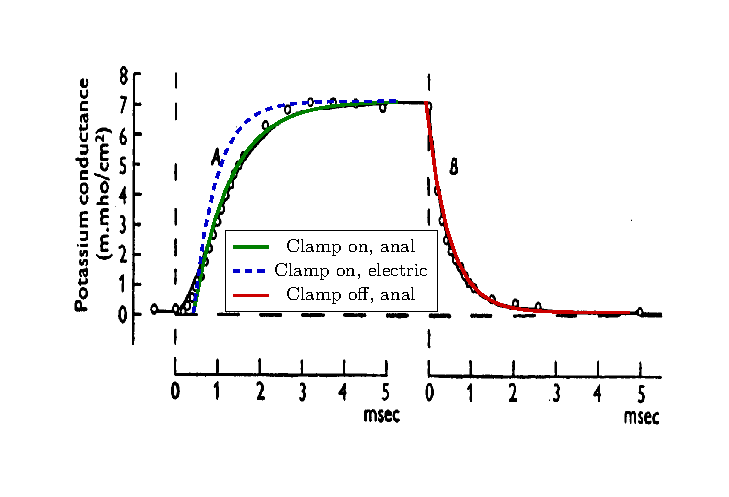
\includegraphics[width=0.95\textwidth]{fig/HodgkinHuxleyFig2Simple.pdf}
	\caption{The measured current, instead of conductance, (Fig.~2 from~\cite{HodgkinHuxley:1952}), demonstrating that two different physical effects result in the rising and falling edge of the measured current.
		\label{fig:HHFig2Simple} }	
\end{figure}



The \textit{slow} input
currents (although due to slightly differing
physical reasons for the different current types) are described by
the following analytic form valid for \textit{fast} currents:
\begin{equation}
	I_{in}=I_{o}*(1-\exp(-\frac{1}{\alpha}*t))*exp(-\frac{1}{\beta}*t)\label{eq:BioCurrentForm}
\end{equation}


\begin{figure}
	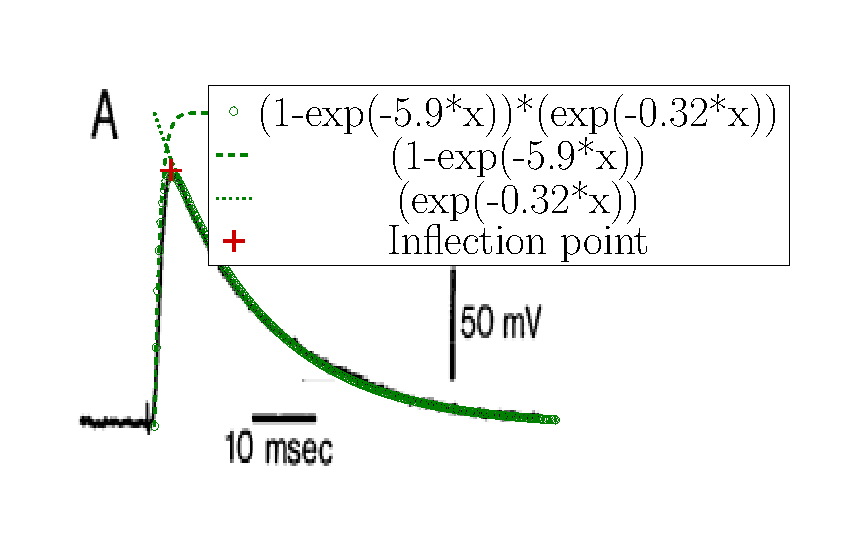
\includegraphics[width=0.95\textwidth]{fig/MasonPSPlin.pdf}
	\caption{The \gls{PSP} shape measured by~\cite{SynapticTransmissionMason:1991} and fitted by function forms
		given by  Eq.(\ref{eq:BioCurrentForm}).
		\label{fig:MasonPSP} }	
\end{figure}

\noindent where $I_{o}$ is the current amplitude per input, and $\alpha$
and $\beta$ are timing constants for current in- and outflow, respectively.
They are (due to geometrical reasons) approximately similar for the
synaptic inputs and differ from the constants valid for the rush-in
current. To implement such an analog circuit with a conventional electronic
circuit, voltage-gated current injectors (with time constants around
1~msec) are needed.
For example, see in Fig~\ref{fig:MasonPSP} the \gls{PSP} measured function shape published in~\cite{SynapticTransmissionMason:1991}, fitted with our theoretical function Eq.(\ref{eq:BioCurrentForm}). The corresponding voltage derivative is as follows:

\begin{equation}
	\frac{dV_{in}}{dt}=\frac{I_{o}}{C}*\biggl(\frac{1}{\alpha}*exp(-\frac{1}{\alpha}*t-\frac{1}{\beta}*t)-\frac{1}{\beta}*exp(-\frac{1}{\beta}*t)*exp(1-exp(-\frac{1}{\alpha}*t))\biggr)\label{eq:PSPderivative}
\end{equation}




\subsection{Condenser\label{sec:Physics-Condenser}}


Cell biochemistry sufficiently well describes the lipid bilayers that constitute the membrane~\cite{OriginOfLifeMicelles:2021,ReproductionLife:2023}.
The negative and positive ends of the lipids that constitute the membrane, in an electrolyte solution, attract and bind ions, forming a charged layer on the membrane surfaces. In this way, the membrane in electrolytes acts as a condenser, comprising two charged sheets on its surfaces, with ill-defined parameters. Their boundaries, thicknesses, and compositions depend on the operating state (unlike conducting plates with well-defined sizes and boundaries). The condenser is not ideal: the charged sheet comprises ions with attached aqueous constituents from the electrolyte, so its thickness is far from the ideal zero thickness of classical electricity. Furthermore, in its wall, it inseparably comprises ion channels (from an electrical point of view: resistors), and the condenser plates are in polarizable electrolyte solutions. 

Cell science does not establish the membrane's electrical phenomena; instead, it attempts to elucidate complex protein activities that explain charge transfer, resting and transient potentials, and explains the entire \textit{biological operation using mathematical formulas without a realistic physical background}. Electrophysiology combines currents of electrons and ions, and \textit{uses Ohm’s Law for its admittedly non-Ohmic systems}. It introduces foreign (clamping) currents into biological systems, attributing their effects to changes in membrane conductance without explaining how \textit{voltage and current can be independent of charge carriers}.


\subsection{Resistor\label{sec:Physics-Resistor}}	

Ions differ from electrons we used to in physical electricity in many features. Their conduction mechanisms
are entirely different, and they are not necessarily present 
in the discussed medium (say, when the medium is surrounded by a charged surface, the field moves free ions out of the volume). They may be produced by biological mechanisms, 
and they are slow (have a couple of $m/s$ speed, creating the illusion
of 'delayed current').
Both disciplines provide an atomic level description, but unfortunately they use the same words for their concepts, although
their meaning can be entirely different. 

In solids, as the Drude model describes, 
electrons constantly bounce among heavier, stationary crystal ions, that make up the structure of the material. With each collision, though, the electron is deflected in a random direction \textit{with a speed that is much larger than the speed gained by the electric field}. The net result is that electrons take a zigzag path due to the collisions, but generally drift in a direction along the electric field. Important, that \textit{the collisions are inelastic}, so the electrons lose (most of) their energy. The solid's gridpoints absorb the energy, which later is released in form of heat. The process is irreversible.

In biological matter, ions convey electricity. So called ion channels
are used for the transfer. Here diffusion and electromigration takes place, by orders of magnitude different speeds. 
The process is mostly reversible. The resistance 
is interpreted as the interaction of charge carriers with the particles in the material that are transported by a driving force (that can comprise also a force of chemical origin).
In solid state, the volume considered is "infinitely large" (that is, the field is homogeneous
and the propagation is isotropic), and the charge carriers are uniform that is only one type of interaction is present.
In biological objects, the volume is more or less limited (is finite), there may be charged objects present that make the propagation non-isotropic. Furthermore, the charge carriers are non-uniform
that introduces thermodynamic interaction in addition to the electrical interaction.
Ions, under the electrical/thermodynamic field (and maybe mechanical constraints) accelerate to the Stokes-Einstein speed (see Eq.(\ref{eq:StokesSpeed})), move against a friction in the electrolyte.
The ions suffer (essentially elastic) collisions with neutral molecules and transfer their momentum (and so: energy) to them. 
From the point of view of ions, the process is energy loss and momentum loss.
From the point of neutral molecules, the process is energy gain and momentum gain. In a free space, the energy and momentum quickly distribute in the entire volume, so the
process in finally irreversible.

If the acceleration occurs in a narrow tube 
such as an ion channel, the wall prevents gaining momentum in the 
direction perpendicular to the direction of acceleration. 
Given that the collisions are elastic, no energy dissipates;
so, in principle, the process is reversible.
Strangely enough, this way the electrical force
accelerates also the neutral molecules; furthermore, their momentum (using an elastic membrane) can fully contribute to the operation
of neuron (forms the \gls{AP}). 

In a narrow tube (such as an ion channel) the momentum exchange
is limited to one direction.
If the ions are accelerated through the channel, due  to the
frequent collisions, they can entirely transfer their 
energy to a large number of neutral molecules. 
Those accelerated molecules having the same speed
may represent a significant "impact force", sufficient
to cause significant mechanical changes throughout
biological systems.
The momentum transfer by collisions
is a two-way process, it is reversible also in the practice. If a small amount of ionized
particles is present in the tube, under an external electrical
field, the charged particles can accelerate the neutral ones.
Vice versa, if the bulk of the particles are moved mechanically (say, when an ultrasound wave
presses the neuron or a rush-in process transfers electric energy to the membrane), the one-directionally moving
neutral molecules transfer momentum to the charged particles,
this way producing measurable electrical waves (such as an \gls{AP}).

The secondary electric quantities can be derived from
the primary quantity: the bulk of the undissociated molecules
'resist' transferring ions under the effect of an electric field (the liquid must be pressed through the tube).
One can measure potential and current along the ion
channel (and so, to calculate resistance), but the behavior of the resistance/conductance is 
drastically different. One has a pneumatic system instead of a voltage generator and the resistance originates in viscosity. Most of the energy is converted to
mechanical energy instead of heat, making the process (mostly) reversible.


The \gls{AP} initially produces an impulse force that compresses the membrane. The compressed membrane, while performing a damped oscillation, pushes and pulls the incompressible electrolyte that contains a small amount of dissociated ions, this way (per defitionem)
creating an observable current and voltage wave. In the 
positive and negative half periods of the elastic oscillation,
due to opposite elastic/pneumatic forces, the current and voltage  change their sign. Given that the charges move at their
Stokes-Einstein speed, the voltage-, current- and pressure waves are synchronized, as observed. The different 
experimental observations measure the same effect
by using their disciplinary measuring devices.

\textit{The energy of the ions cannot dissipate; instead, the neutral and charged 
particles share it}, and convert between kinetic and elastic energies (the electric energy is much smaller).
That is, the 
neuron can produce heat in the positive phase of the
elastic oscillation (the electrolyte is compressed),
and can reabsorb heat in the negative phase (decompression), in full accordance with the correctly interpreted laws of physics.
\index{heat absorption by neuron}
This way, by introducing the correct interpretation of "resistance" for ion channels, the seven-decades-old
contradiction~\cite{HeatProductionNeuron:1958}
between the electrical and thermodynamic observations
are finally resolved, furthermore, the conflicting theories
can be naturally unified.

